\section{Related work}
\label{sec:related_work}
%
To start with, let us refine requirements R1$,\ldots,$R4.

\noindent{\textbf{R1:}} The technique should rapidly create an unobstructed view of the target, \emph{i.e.}, such a view should be created at interactive frame rates (10 fps or more) with no special pre-processing of the input volume (\emph{e.g.}, segmentation), and with minimal user input (\emph{e.g.}, using simple mouse and/or keyboard-modifier events). All above are needed to ensure that one can freely \emph{explore} the volume by activating the lens anywhere with minimal effort and seeing its effect in real-time.

\noindent{\textbf{R2:}} Allowing a flexible exploration of the target zone means that one can manipulate the zone in the lens in various ways to see how the target is actually embedded in its surrounding context.

\noindent{\textbf{R3:}} Keeping the context means that the visualization around the lens does not change significantly from what would be shown there if the lens were not activated. This is needed to maintain the user's mental map before \emph{vs} after activating the lens.

\noindent{\textbf{R4:}} The lens should enable the exploration of datasets where targets cannot be easily separated (isolated) from their surrounding context simply by manipulating parameters of the transfer functions (TF). One such issue is when targets and surrounding zones have similar densities; in this case, using a single global opacity TF could either render everything opaque (thus, it will be hard to visually isolate the target) or highly transparent (thus, the zone around the target will be transparent but so will be the target too).

Previous work on handling occlusion when exploring volume data can be divided into occlusion management techniques and lenses-and-deformation techniques. We next discuss these and also point out limitations from the perspective of R1$,\ldots,$R4.

\begin{figure*}[htbp]
\centering
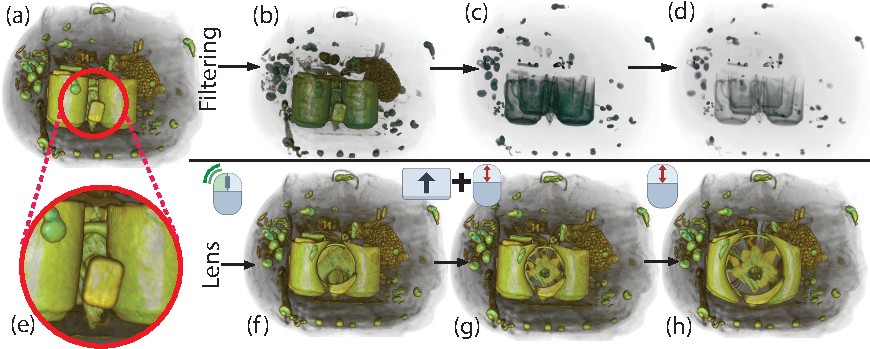
\includegraphics [width=0.9\textwidth]{shuriken.eps}
\vspace{-0.15cm}
\caption{(a-c) A baggage scan is viewed from different angles. In view (c), a suspicious sharp object is spotted between a set of mugs. (d-f) Filtering densities using a classical 1D opacity transfer function removes progressively more of the occluders (mugs), but also the target. (g) The user applies the lens on the target object (double-click). An animation starts opening the lens, rays are gathered to pass through occluders. Halfway through the animation, the object is magnified, but only the area close to the lens is visible. (h) The fish-eye field of view at the end of the animation scatters rays to fully show the target. (i) The lens is increased to magnify the target (mouse scroll).}
\label{f:baggage_lens}
\end{figure*}
\vspace{-0.15cm}


\subsection{Occlusion management}
%
Many occlusion management approaches have been proposed\,\cite{4483791}. Multiple viewports show the data from different perspectives\,\cite{WangBaldonado:2000:GUM:345513.345271}. This does not help when the target is strongly occluded from \emph{all} possible viewpoints (R4). Virtual X-ray methods make targets visible by turning occluders (half-)transparent\,\cite{Burns:2008:ACC:1457515.1409107}. Kruger et al.\,\cite{4015450} proposed ClearView, which interactively focuses on specific areas in the data while preserving context without visual clutter by modulating transparency. Correa and Ma\,\cite{5416704} proposed visibility-driven transfer functions (TFs) to maximize the visibility of selected data-intervals. Designing good TFs is still challenging (R2) in general: For instance, in baggage inspection, a dissimulation strategy is to hide a threat among same-density objects, so TF editing cannot easily remove occluders but keep the target (R4)\,\cite{7819413}. De-occluding a tumor from surrounding similar-density tissue in medical scans is a similar situation\,\cite{CGF:CGF12927}. 
Rezk-Salama and Kolb\,\cite{CGF:CGF979} also considered the voxels' occurrence on the cast ray, besides their densities and positions. Hurter et al.\,\cite{moleview,6787171} removed occluders in 2D images, volumes, and trail-sets by deforming (pushing them away) in a focus area. Occludes are selected based on data value-ranges, thus we have here the same limitation as ClearView (R4). Li et al.\,\cite{Li:2012:LVV:2425296.2425325} proposed luggage virtual unpacking where targets are cleared by interactively moving away occluders. This, however, alters the \emph{context} (relative position, connectivity) where occluders occur (R3). Recently, an interactive volumetric data exploration via direct voxel manipulation was proposed\,\cite{7819413}. Extending such approaches in a DVR setting to more complex deformations or changes of the data-in-focus is computationally challenging (R1).

\vspace{-0.15cm}
\subsection{Lenses and deformations}
%
An interactive lens is a lightweight tool to solve localized visualization problems by temporarily altering a selected part of the visual data representation\,\cite{CGF:CGF12871}, and hence provides focus-and-context (F+C) solutions to volumetric data occlusion (R2). Parametrizable lens properties include position, shape, appearance, size, orientation, and selection of included data (focus). The lens \emph{shape} is usually chosen to meet the requirements of the application and is linked to the lens function. Most lenses are circular\,\cite{1648236} (a design we also choose), rectangular\,\cite{Kincaid:2010:SFA:1907651.1907963}, or adapt their shape to the data-in-focus\,\cite{Pindat:2012:JCA:2380116.2380150,Thiede2008}. The lens \emph{position} and \emph{size} can be changed manually by the user, or automatically to guide users toward interesting events in the data\,\cite{Tominski:2011:ECU:2336207.2336211} or along a path of interesting events\,\cite{Alvina:2014:RER:2598153.2598200}. Our lens updates automatically its properties once a target has been selected. This allows a smooth transition towards an unobstructed and magnified area of interest.

Lenses for DVR face spatial selection and occlusion challenges. Magic Lens\,\cite{1532818} addresses these by rendering occlusions with lower opacity and magnifying pre-computed features interactively or automatically in a pre-segmented dataset. This, however, does not provide an (interactive) way to deal with similar-density occluders and targets (R4) and does not propose local exploration of the target context (R2). GlyphLens\,\cite{7539643} removes occluding glyphs by pulling them aside through animation. However, this covers only glyph-based and not DVR visualizations. 

Lenses can create discontinuities between their inside and outside areas. Deformations can be a solution to this.
Hsu et al.\,\cite{Hsu:2011:RFM:2070781.2024165} create flexible deformations by non-linearly sampled rays to smoothly project objects at multiple levels of detail. However, this is computationally expensive and far from real-time (R1). Exploded views are used to partition a volume into several segments\,\cite{Sonnet:2004:IEA:989863.989871,4015467}. This strongly reduces occlusion but distorts the context (R3) and requires some sort of data pre-segmentation which takes time to compute (R1). Correa et al.\,\cite{Correa:2007:IDD:1313046.1313163,Correa:2006:FAV:1187627.1187827} allow one to manipulate the geometry of a data object. McGuffin et al.\,\cite{1250400} performed deformations using peeling to see hidden parts of the data. Such techniques remove potentially important contextual information surrounding the target, which makes it hard to see how the target is embedded in its context (R2).

Deformations can reveal specific data features by using a precomputed segmentation. Tong et al. proposed a deforming lens which moves streamlines to observe the inner part of streamline bundles\,\cite{7332955}. Other techniques performed deformations using surgical metaphors\,\cite{4069230,Correa:2006:FAV:1187627.1187827} to show hidden parts of a volume. Such techniques do not offer tools for local manipulation of the viewpoint that allows seeing a target under multiple perspectives (R2) while keeping the global context. 

Using non-straight-line rays is another way to avoid occluders. Cui \emph{et al.}\,\cite{cui10} propose curved (B{\'e}zier) rays to support this. Wu \emph{et al.}\,\cite{wu16} refine this further to create multi-perspective views. These approaches require a quite careful ray-path planning in advance, so they are not directly aimed at a lens effect (R2). Also, the target should be accessible from the viewpoint via a (possibly curved) path (R4). Also, from the presented examples, although two examples of DVR models are given, it seems these techniques mainly address de-occlusion in large 3D polygonal scenes such as terrain and city models.

Table~\ref{tab:methods} summarizes the main advantages and limitations of a set of volumetric exploration techniques selected from the ones mentioned above which are close to our proposal. As visible, none of the techniques scores high on all requirements. The table also lists the number of different datasets and/or use-cases these techniques were tested on. We will validate our proposal on a similar number of use-cases (Sec.~\ref{sec:scenarios}).
\begin{table}[htbp]
\centering
\small
\begin{tabular}{ |c|c|c|c|c|c| }
\hline
\textbf{Technique} & \textbf{R1} & \textbf{R2} & \textbf{R3} & \textbf{R4} & \textbf{Use-cases}\\
\hline
\hline
McGuffin \emph{et al.}\,\cite{1250400} & \CIRCLE & \Circle & \CIRCLE & \CIRCLE & 1\\
Sonnet \emph{et al.}\,\cite{Sonnet:2004:IEA:989863.989871} & \LEFTcircle & \Circle & \CIRCLE & \LEFTcircle & 5\\
Wang \emph{et al.}\,\cite{1532818} & \CIRCLE &  \Circle & \CIRCLE & \LEFTcircle & 6\\
Bruckner \emph{et al.}\,\cite{4015467} & \LEFTcircle &  \Circle &  \Circle & \CIRCLE & 6\\
Correa \emph{et al.}\,\cite{Correa:2007:IDD:1313046.1313163,Correa:2006:FAV:1187627.1187827} & \CIRCLE & \Circle & \CIRCLE & \CIRCLE & 8\\
Cui \emph{et al.}\,\cite{cui10} & \CIRCLE &  \Circle & \CIRCLE &  \Circle & 5\\
Hsu \emph{et al.}\,\cite{Hsu:2011:RFM:2070781.2024165} &  \Circle & \LEFTcircle & \CIRCLE & \CIRCLE & 4\\
Hurter \emph{et al.}\,\cite{6787171} & \CIRCLE & \LEFTcircle & \CIRCLE &  \Circle & 6\\
Wu \emph{et al.}\,\cite{wu16} & \CIRCLE &  \Circle & \CIRCLE &  \Circle & 5\\
\hline
\end{tabular}
\caption{Related work selection \emph{vs} requirements R1..R4 ($\CIRCLE$: good, $\LEFTcircle$: average, $\Circle$: limited) and the number of use-cases (datasets) used in the respective studies to demonstrate these methods.}
\label{tab:methods}
\end{table}



\vspace{-0.09cm}
\subsection{Detailed contributions}
%
Summarizing the above discussion on the requirements and related work on occlusion management, we propose a new technique which combines high-quality DVR with a fast, versatile, and easy to use, lens to support the interactive exploration of occluded data in volumes. In the classification of view deformations by Carpendale \emph{et al.}\,\cite{595268}, we use a nonlinear radial distortion through an interactive lens to remove occluding items and keep the global context while magnifying a partially occluded item. Related to volumetric lens techniques, we frame our contribution as follows: We propose an interactive deforming lens that magnifies and pushes aside occluding objects located in front of a designated focal point which meets the four requirements; the combination of flexible and real-time interactive changing of the focal point, custom bent rays used for DVR, lens deformation, and shading and transfer function in the focus area allow us to provide \emph{on the fly} a range of perspectives of the targets, without having to change the viewpoint or manipulate complex parameters in multiple linked views.


